\newpage

\chapter{Apêndice 3}
\label{apendice3}

\section{Pesquisa com profissionais de software livre e métodos ágeis}

	Foi realizada uma pesquisa para entender o que profissionais que trabalham com software livre e métodos ágeis entendem sobre as técnicas de usabilidade. O resultado se encontram abaixo:
	
	A grande maioria dos profissionais pesquisados eram desenvolvedores, seguidos de designs, arquitetos de informação, especialistas de usabilidade e gerentes de projetos. Alguns deles realizam mais de um papel em sua equipe de trabalho.
	
	\begin{figure}[!h]
    	\centering
    	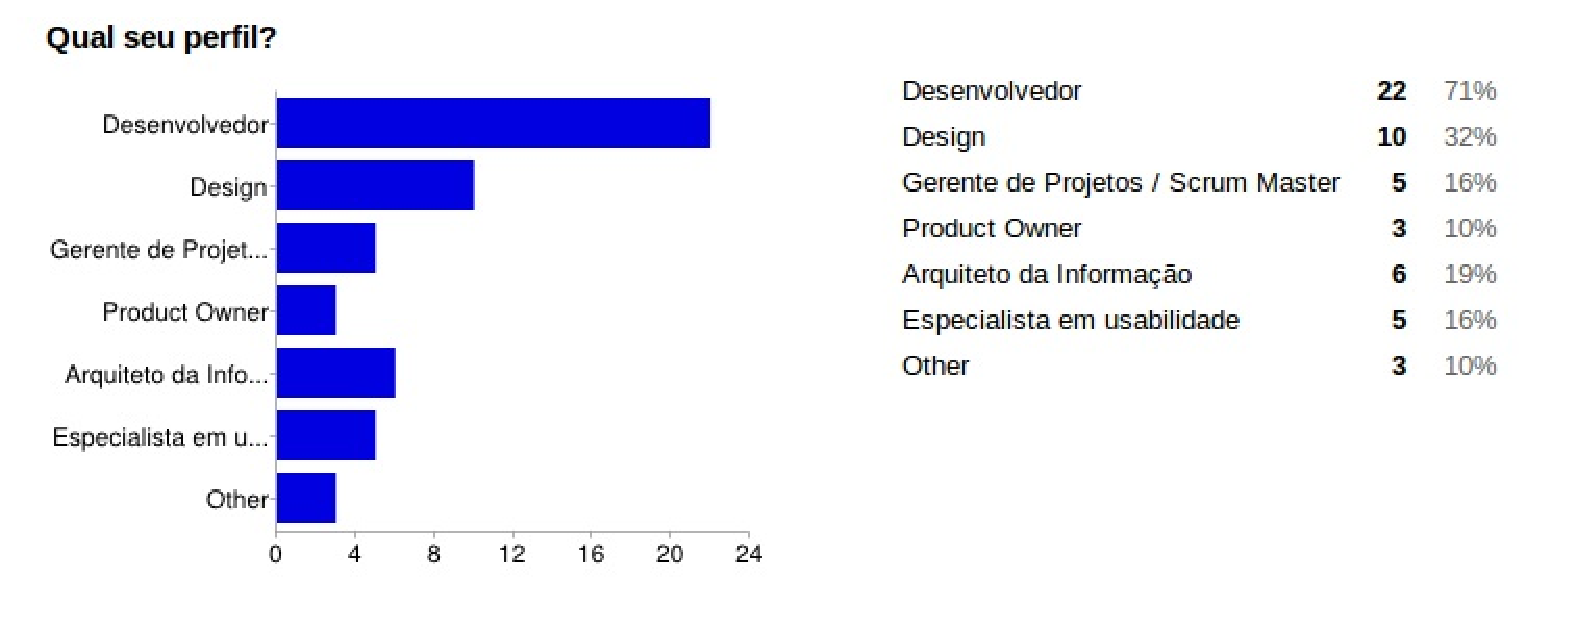
\includegraphics[keepaspectratio=true,scale=0.55]
      		{figuras/perfil.eps}
    	\label{concepcao}
		\caption{Perfil dos entrevistados}
	\end{figure}
	
	Como a pesquisa foi realizada com profissionais diversos, alguns não estavam envolvidos com software livre e com métodos ágeis simultâneamente. Dentre os pesquisados a grande maioria, 48\% tinham entre 1 e 2 anos de experiência com métodos ágeis. Em relação à software livre, 19\% entre 1 e 2 anos, 19\% de 5 a 10 anos e 19\% não trabalhavam com software livre.
	
	\begin{figure}[!h]
    	\centering
    	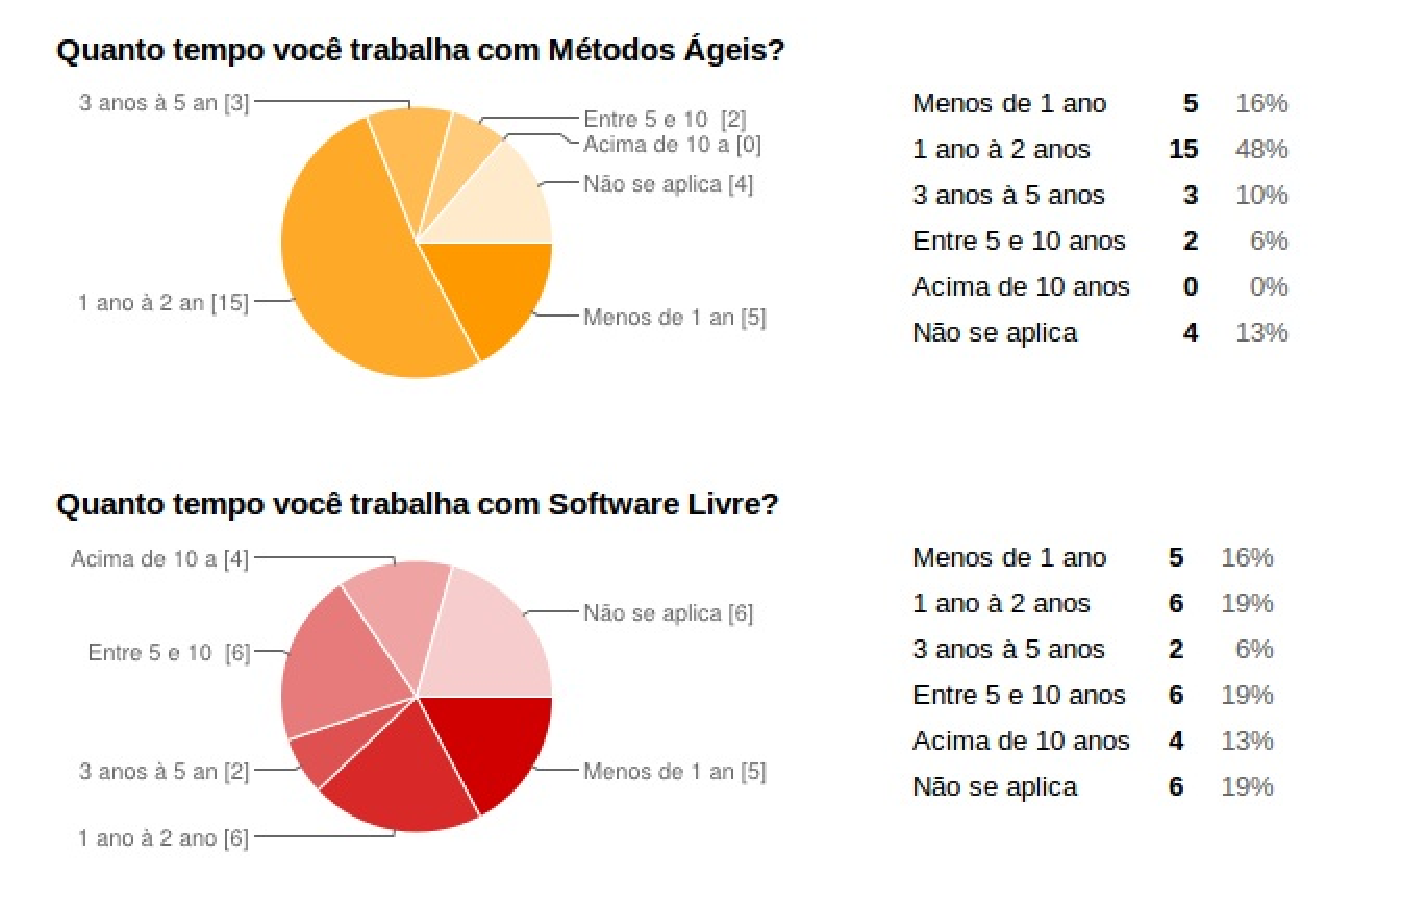
\includegraphics[keepaspectratio=true,scale=0.55]
      		{figuras/tempo_trabalho.eps}
    	\label{concepcao}
		\caption{Tempo de trabalho}
	\end{figure}			
	\begin{figure}[!h]
    	\centering
    	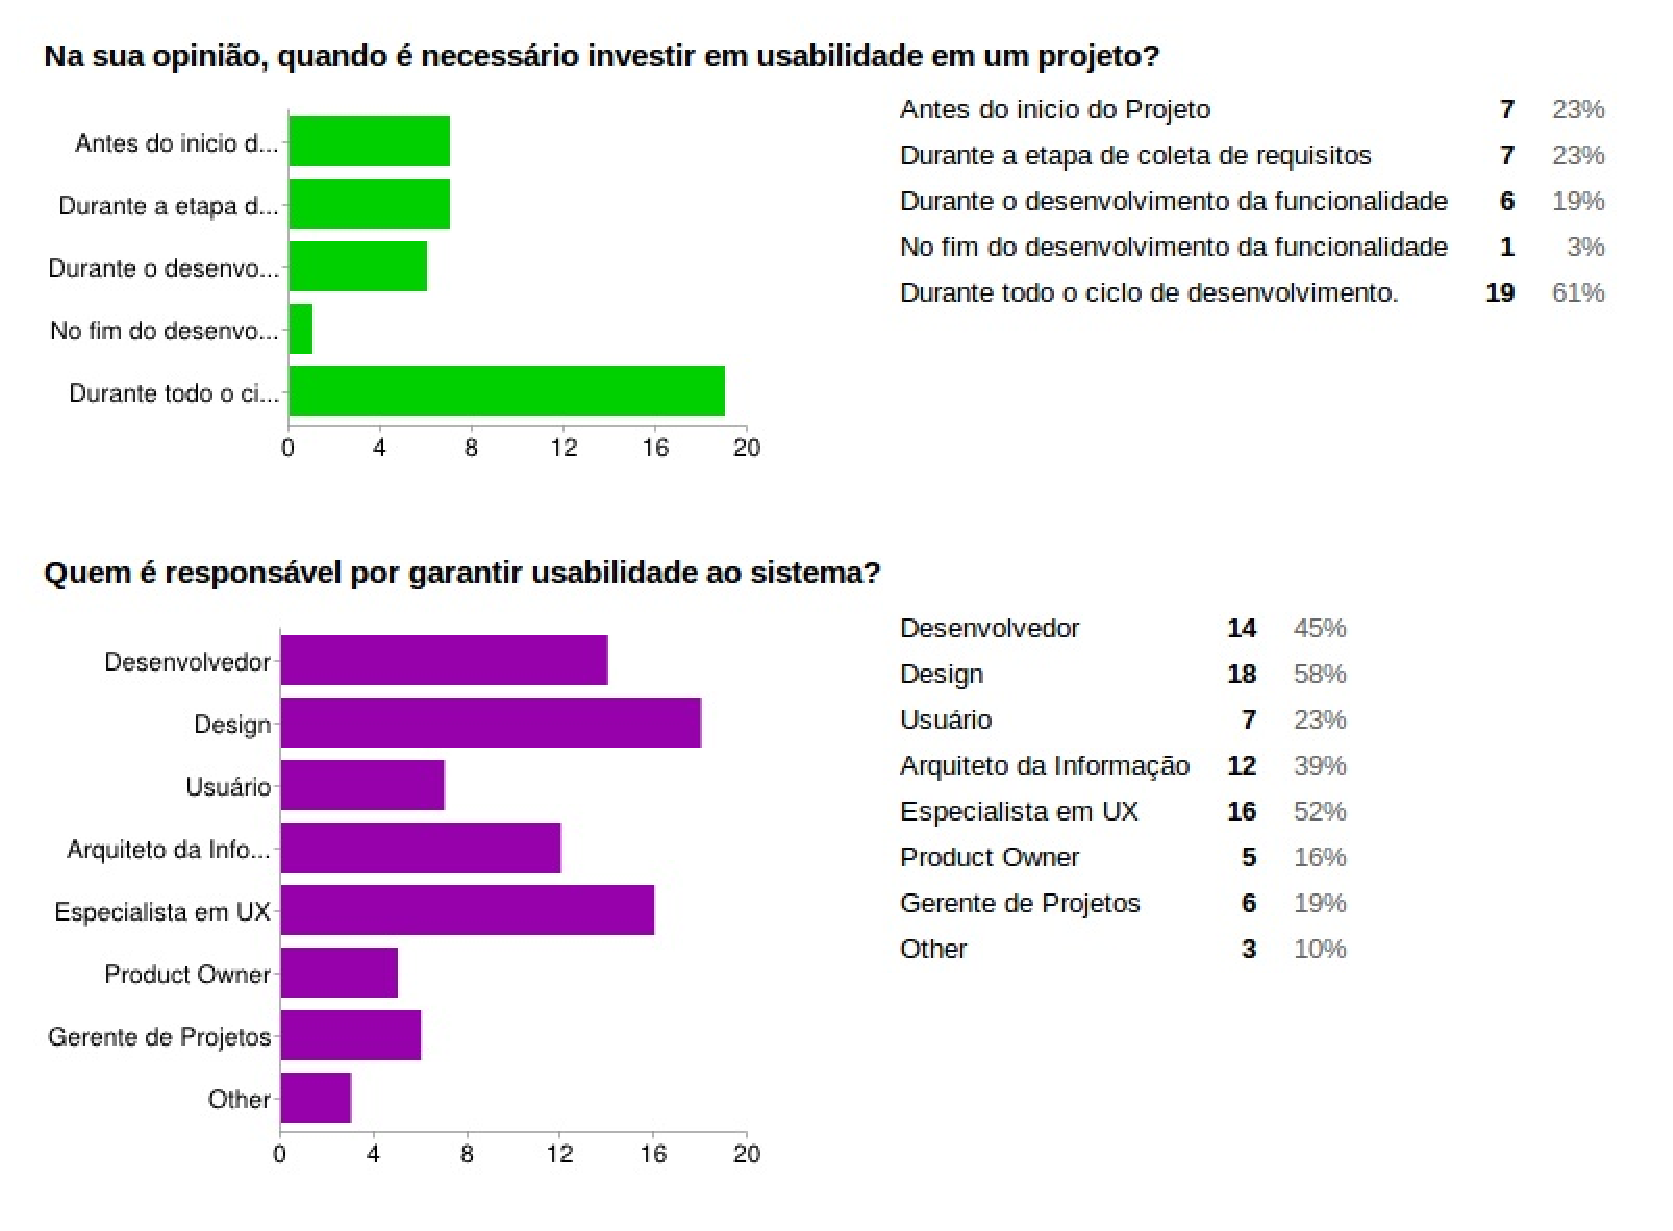
\includegraphics[keepaspectratio=true,scale=0.55]
      		{figuras/quando_e_quem.eps}
    	\label{concepcao}
		\caption{Quando e quem é responsável por garantir a usabilidade}
	\end{figure}

Para 61\% dos entrevistados, investir em usabilidade deve ser feito em todo o ciclo de desenvolvimento e realizada não somente pelos especialistas de usabilidade, mas também pelos desenvolvedores e designs.

\newpage

	Os resultados abaixo mostram as técnicas utilizadas pelos profissionais para avaliar, análisar e conceber interfaces com usabilidade.
	
	\begin{figure}[!h]
    	\centering
    	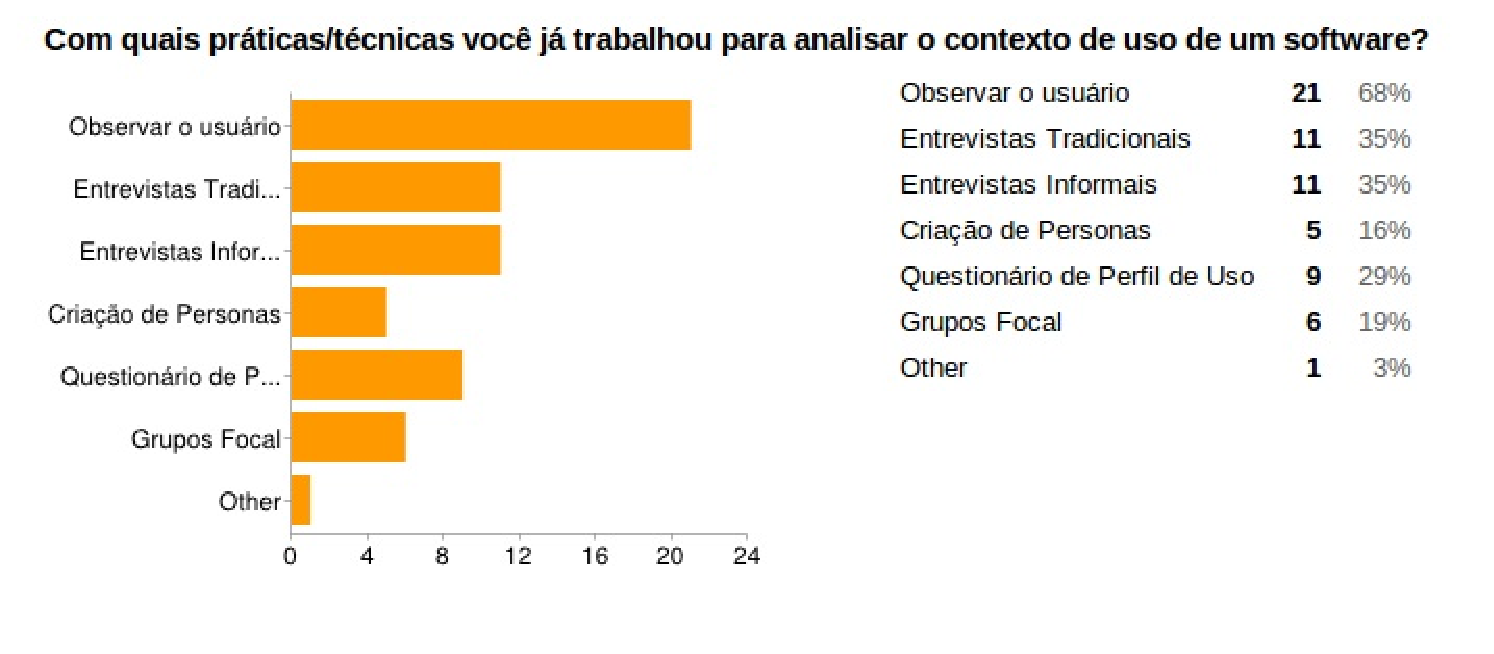
\includegraphics[keepaspectratio=true,scale=0.55]
      		{figuras/contexto_uso.eps}
    	\label{concepcao}
		\caption{Técnicas de contexto de uso}
	\end{figure}
	
	Uma das técnicas mais utilizadas para análisar o contexto de uso do sistema são as observações de usuários, com 68\%, as entrevistas estão em seguidas com 35\% e os questionários de perfil de uso com 29\%.
	
	\begin{figure}[!h]
    	\centering
    	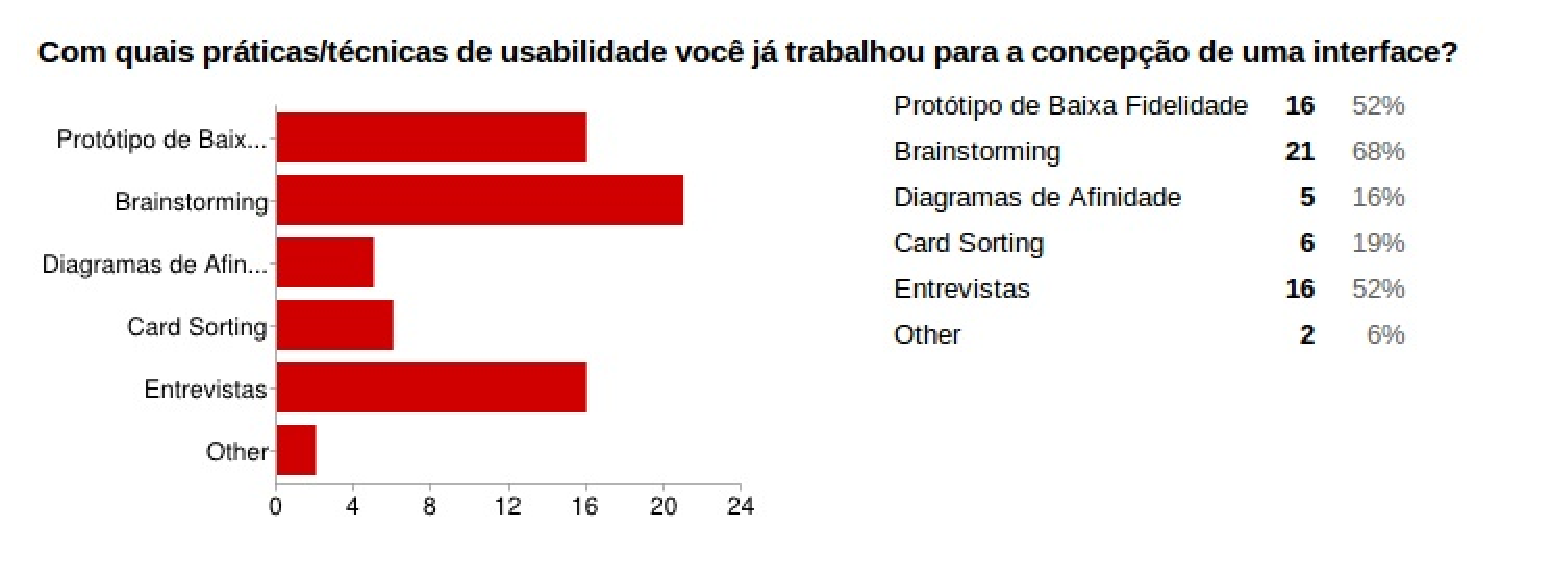
\includegraphics[keepaspectratio=true,scale=0.55]
      		{figuras/tecnica_concepcao.eps}
    	\label{concepcao}
		\caption{Técnicas de concepção de interfaces}
	\end{figure}
	
	A técnica de Braistorming é bastante utilizada por 68\% dos pesquisados para concepção de novas interfaces. Os protótipos de baixa fidelidade são bastante utilizados pelos pesquisados. 52\% também realizam entrevistas com usuários quando necessitam criar uma nova interface.
		
	\begin{figure}[!h]
    	\centering
    	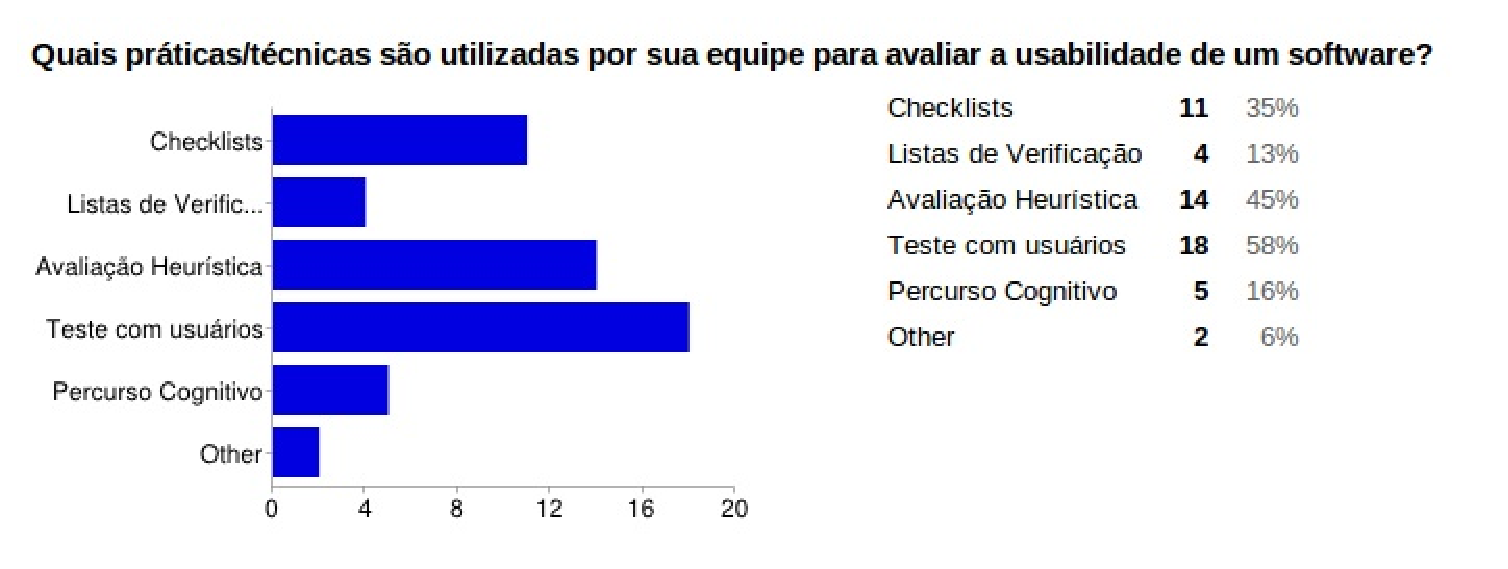
\includegraphics[keepaspectratio=true,scale=0.55]
      		{figuras/avaliacao_usada.eps}
    	\label{concepcao}
		\caption{Técnicas de avaliação utilizadas}
	\end{figure}	
	
	Os testes com usuários é uma das técnicas mais utilizadas pelos profissionais com 58\%, seguido pelas técnicas de avaliação heurísticas e checklists (listas de verificação). 
	
	Os resultados abaixo mostram qual a importância de cada técnica de concepção de uma interface de acordo com a percepção dos pesquisados.
	
	\begin{figure}[!h]
    	\centering
    	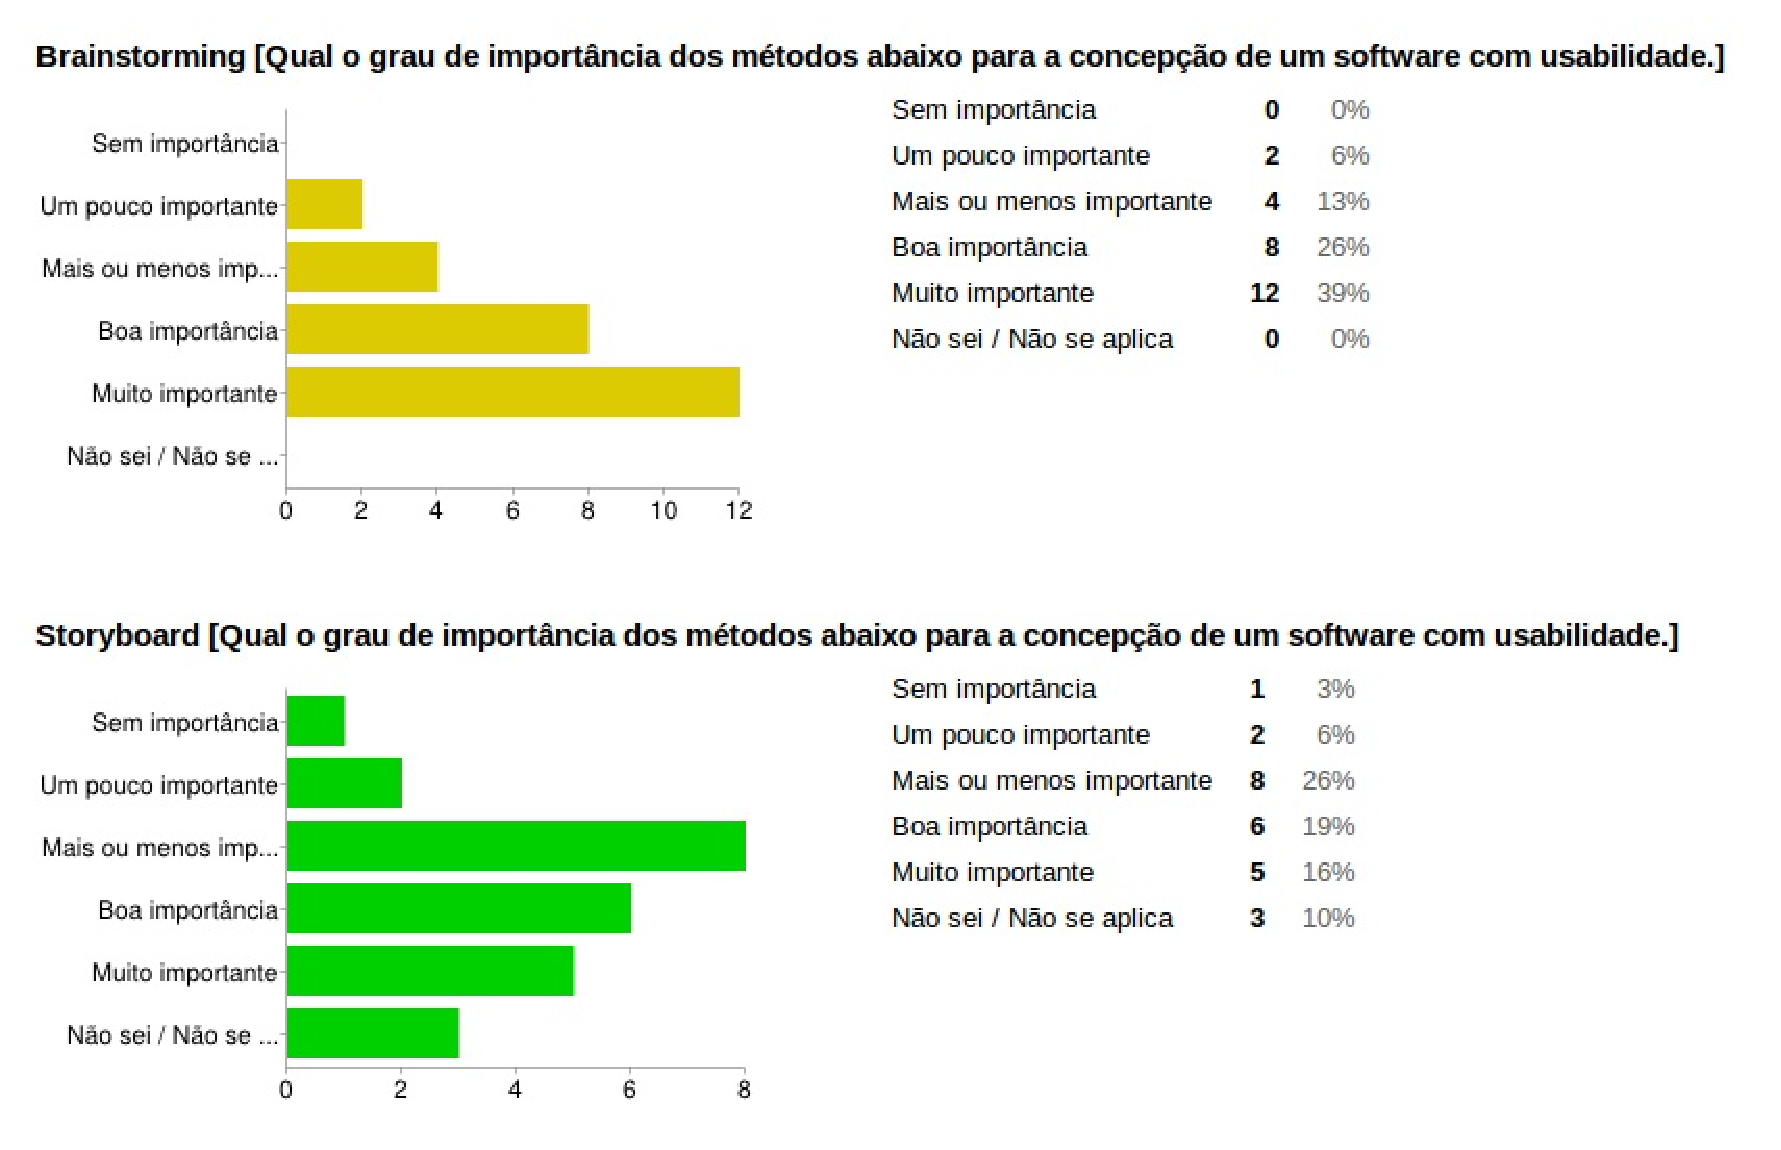
\includegraphics[keepaspectratio=true,scale=0.55]
      		{figuras/concepcao1.eps}
    	\label{concepcao}
		\caption{Técnicas de concepção - Brainstorming e Storyboard}
	\end{figure}
	
	Em relação ao Brainstorming, 39\% dos entrevistados concordam que a técnica é muito importante, já em relação ao storyboard a maioria, 26\% informa que é mais ou menos importante. 
	
	\begin{figure}[!h]
    	\centering
    	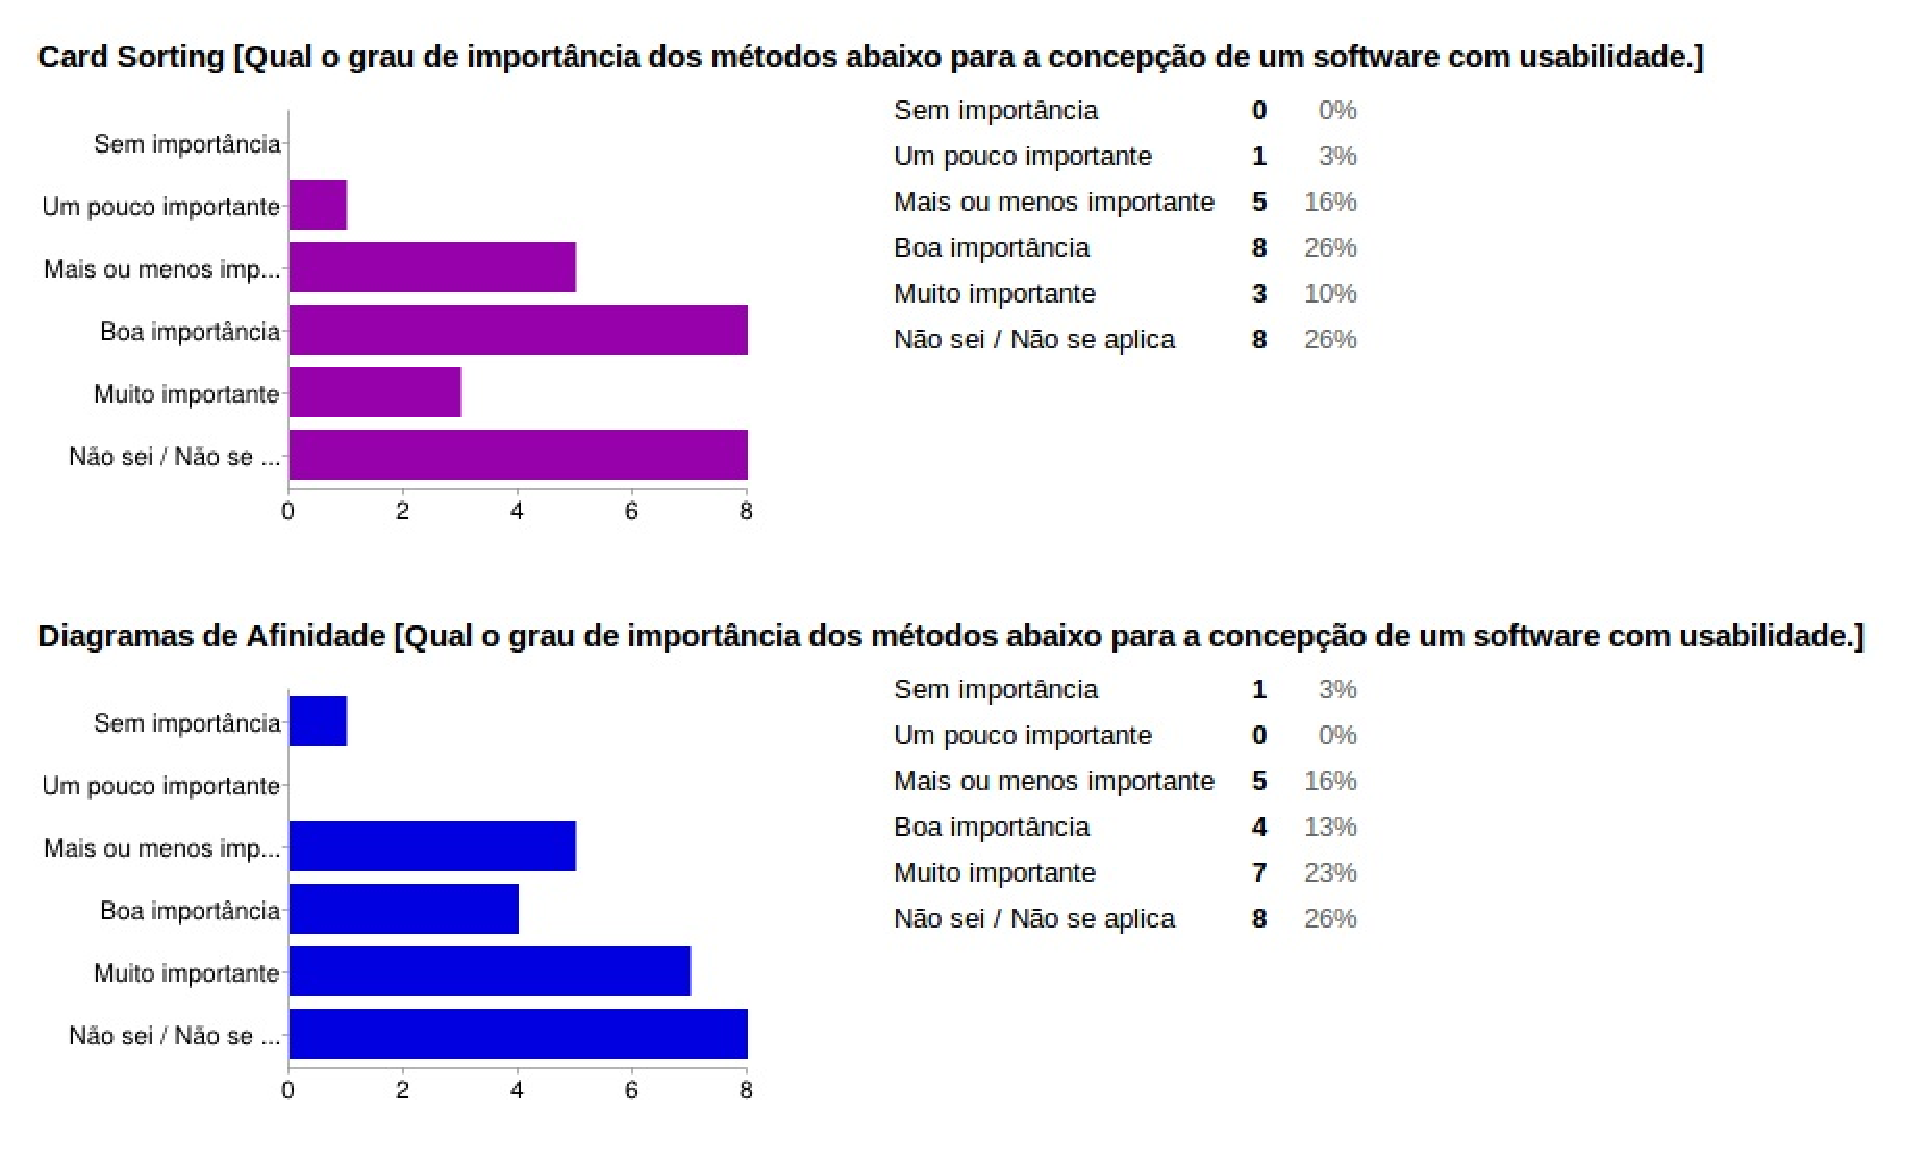
\includegraphics[keepaspectratio=true,scale=0.55]
      		{figuras/concepcao2.eps}
    	\label{check04}
		\caption{Técnicas de concepção - Card Sorting e Diagramas de Afinidade}
	\end{figure}

	Em relação as técnicas de Card Sorting e Diagramas de afinidade, 26 por cento dos pesquisados não sabiam o que eram cada técnica. 
		
	\begin{figure}[!h]
    	\centering
    	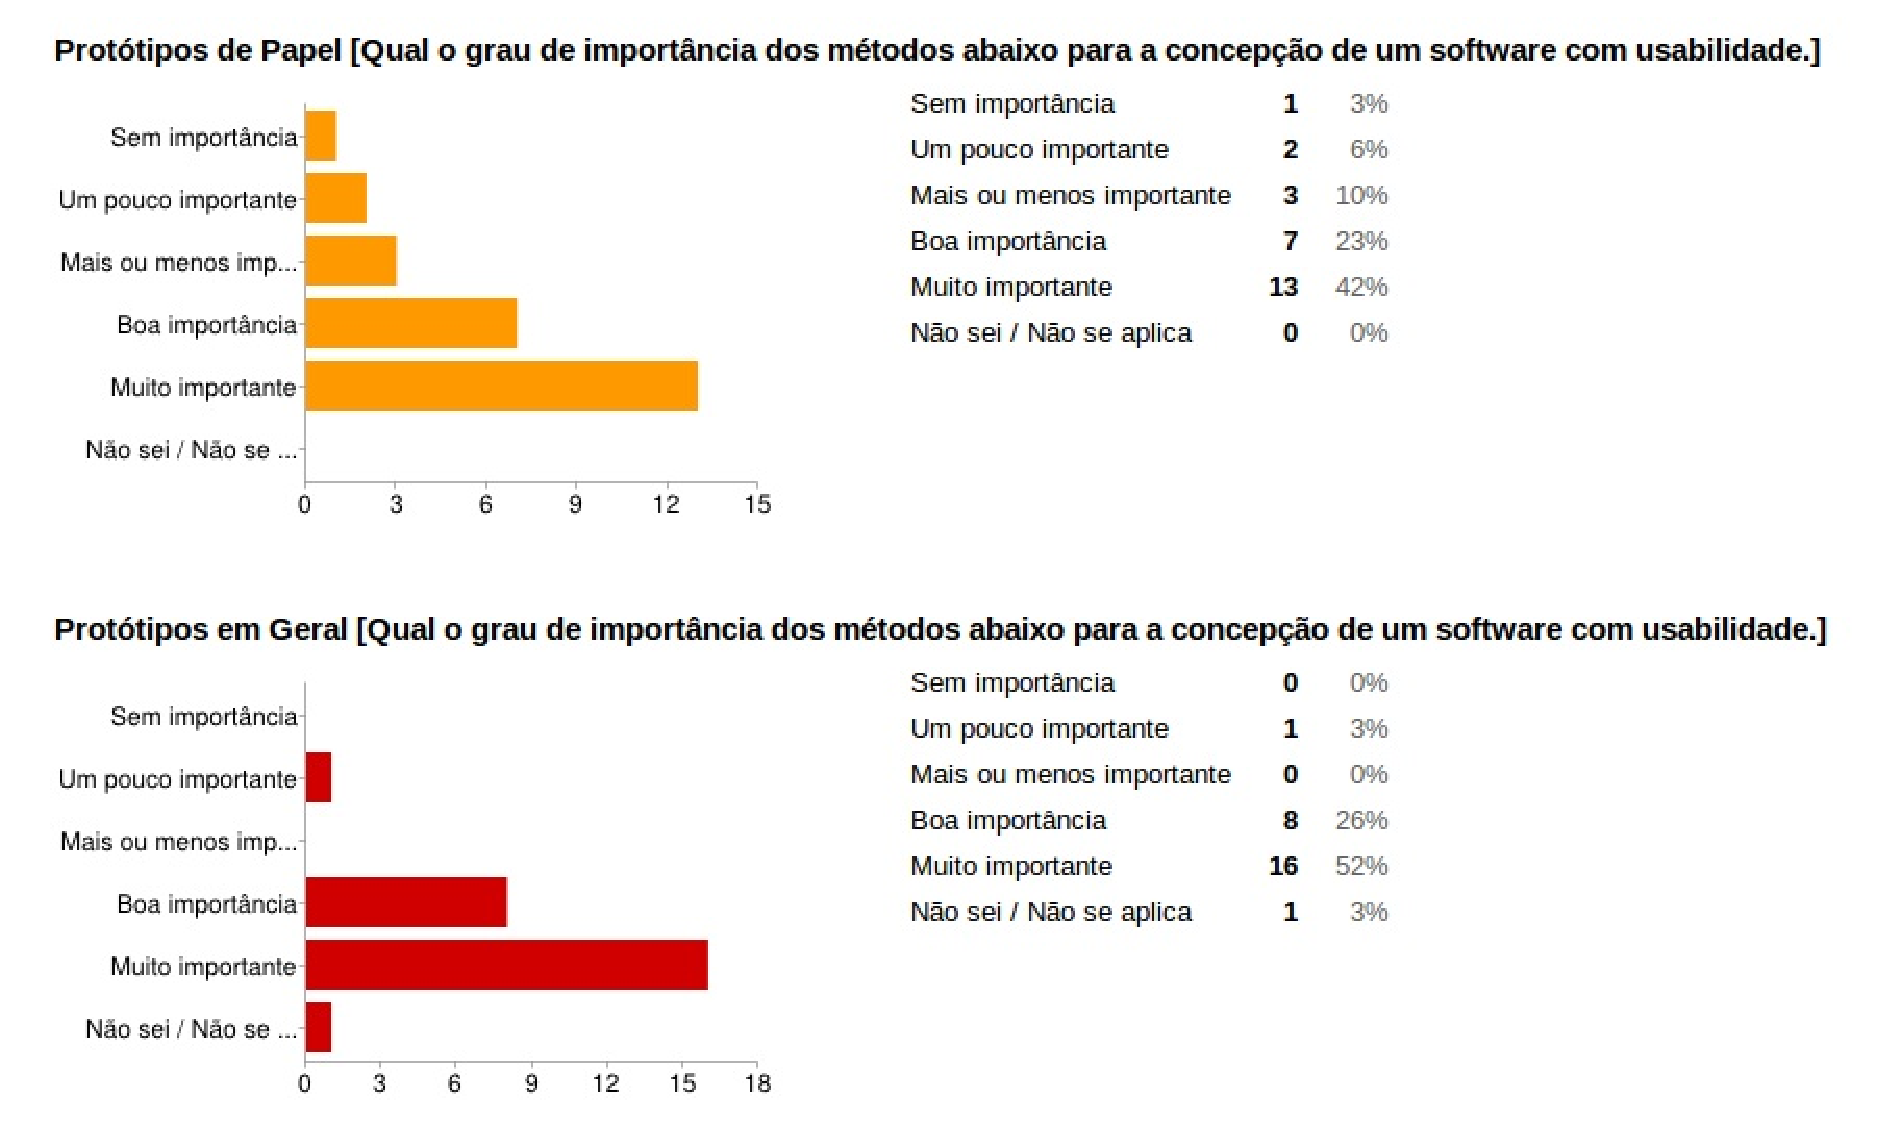
\includegraphics[keepaspectratio=true,scale=0.55]
      		{figuras/concepcao3.eps}
    	\label{check04}
		\caption{Técnicas de concepção - Protótipos}
	\end{figure}
	
	As técnicas de prototipação seja de baixa fidelidade ou geral obtiveram uma boa aceitação por parte dos pesquisados.

\newpage

	Os resultados abaixo mostram a importância das técnicas de análise.
	
	\begin{figure}[!h]
    	\centering
    	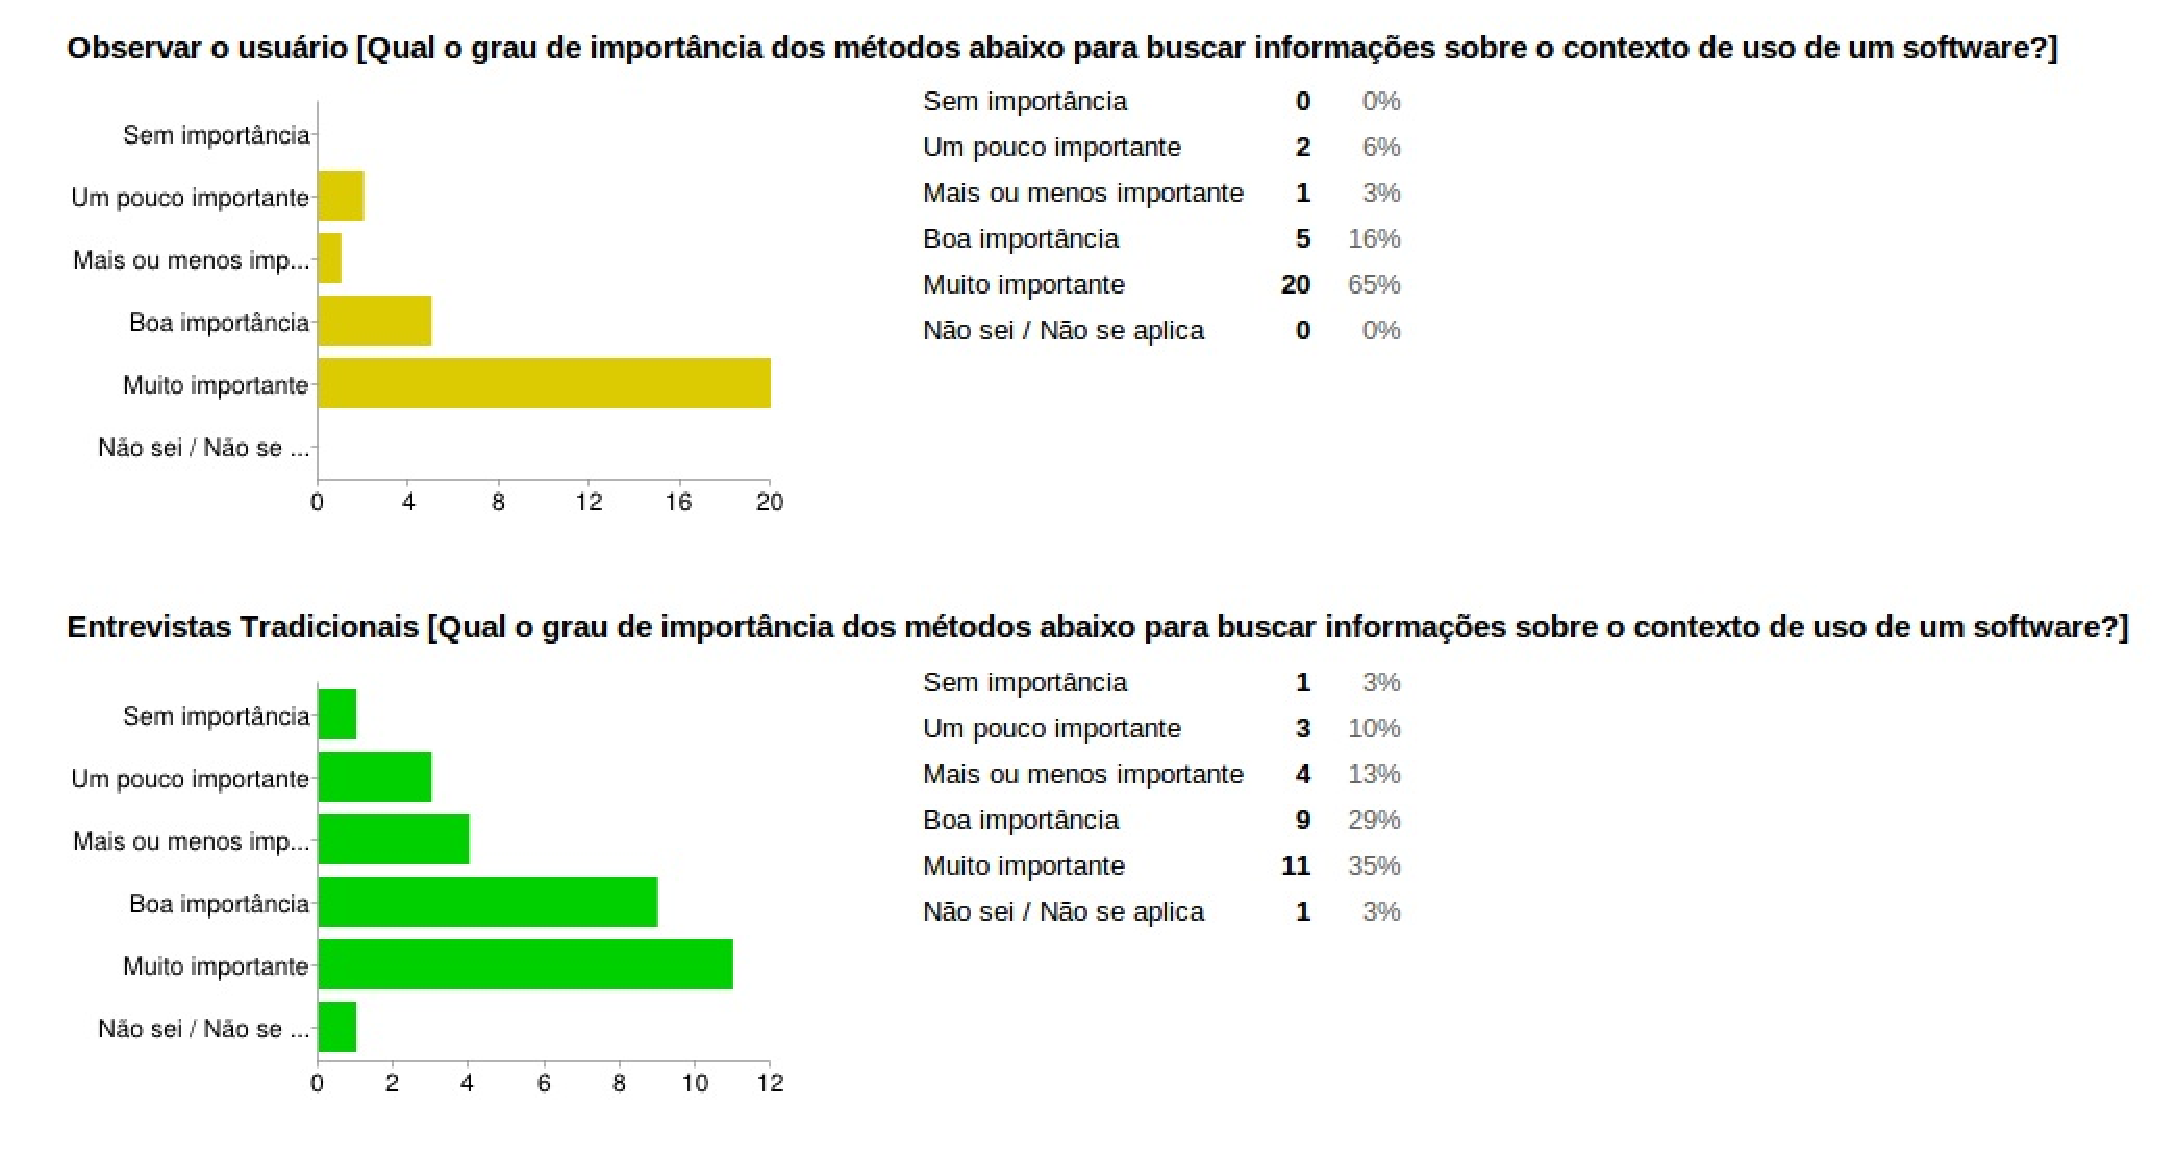
\includegraphics[keepaspectratio=true,scale=0.50]
      		{figuras/analise1.eps}
    	\label{check04}
		\caption{Técnicas de análise - Observação e entrevistas tradicionais}
	\end{figure}
	
	As técnica de observar o usuário obteve uma grande aceitação por parte dos pesquisados, sendo 65\% tendo muita importância.
	 
	As entrevistas tanto tradicionais, como as informais obtiveram resultados pŕoximos, mais de 50\% informaram que têm boa ou muita importância.
		
	\begin{figure}[!h]
    	\centering
    	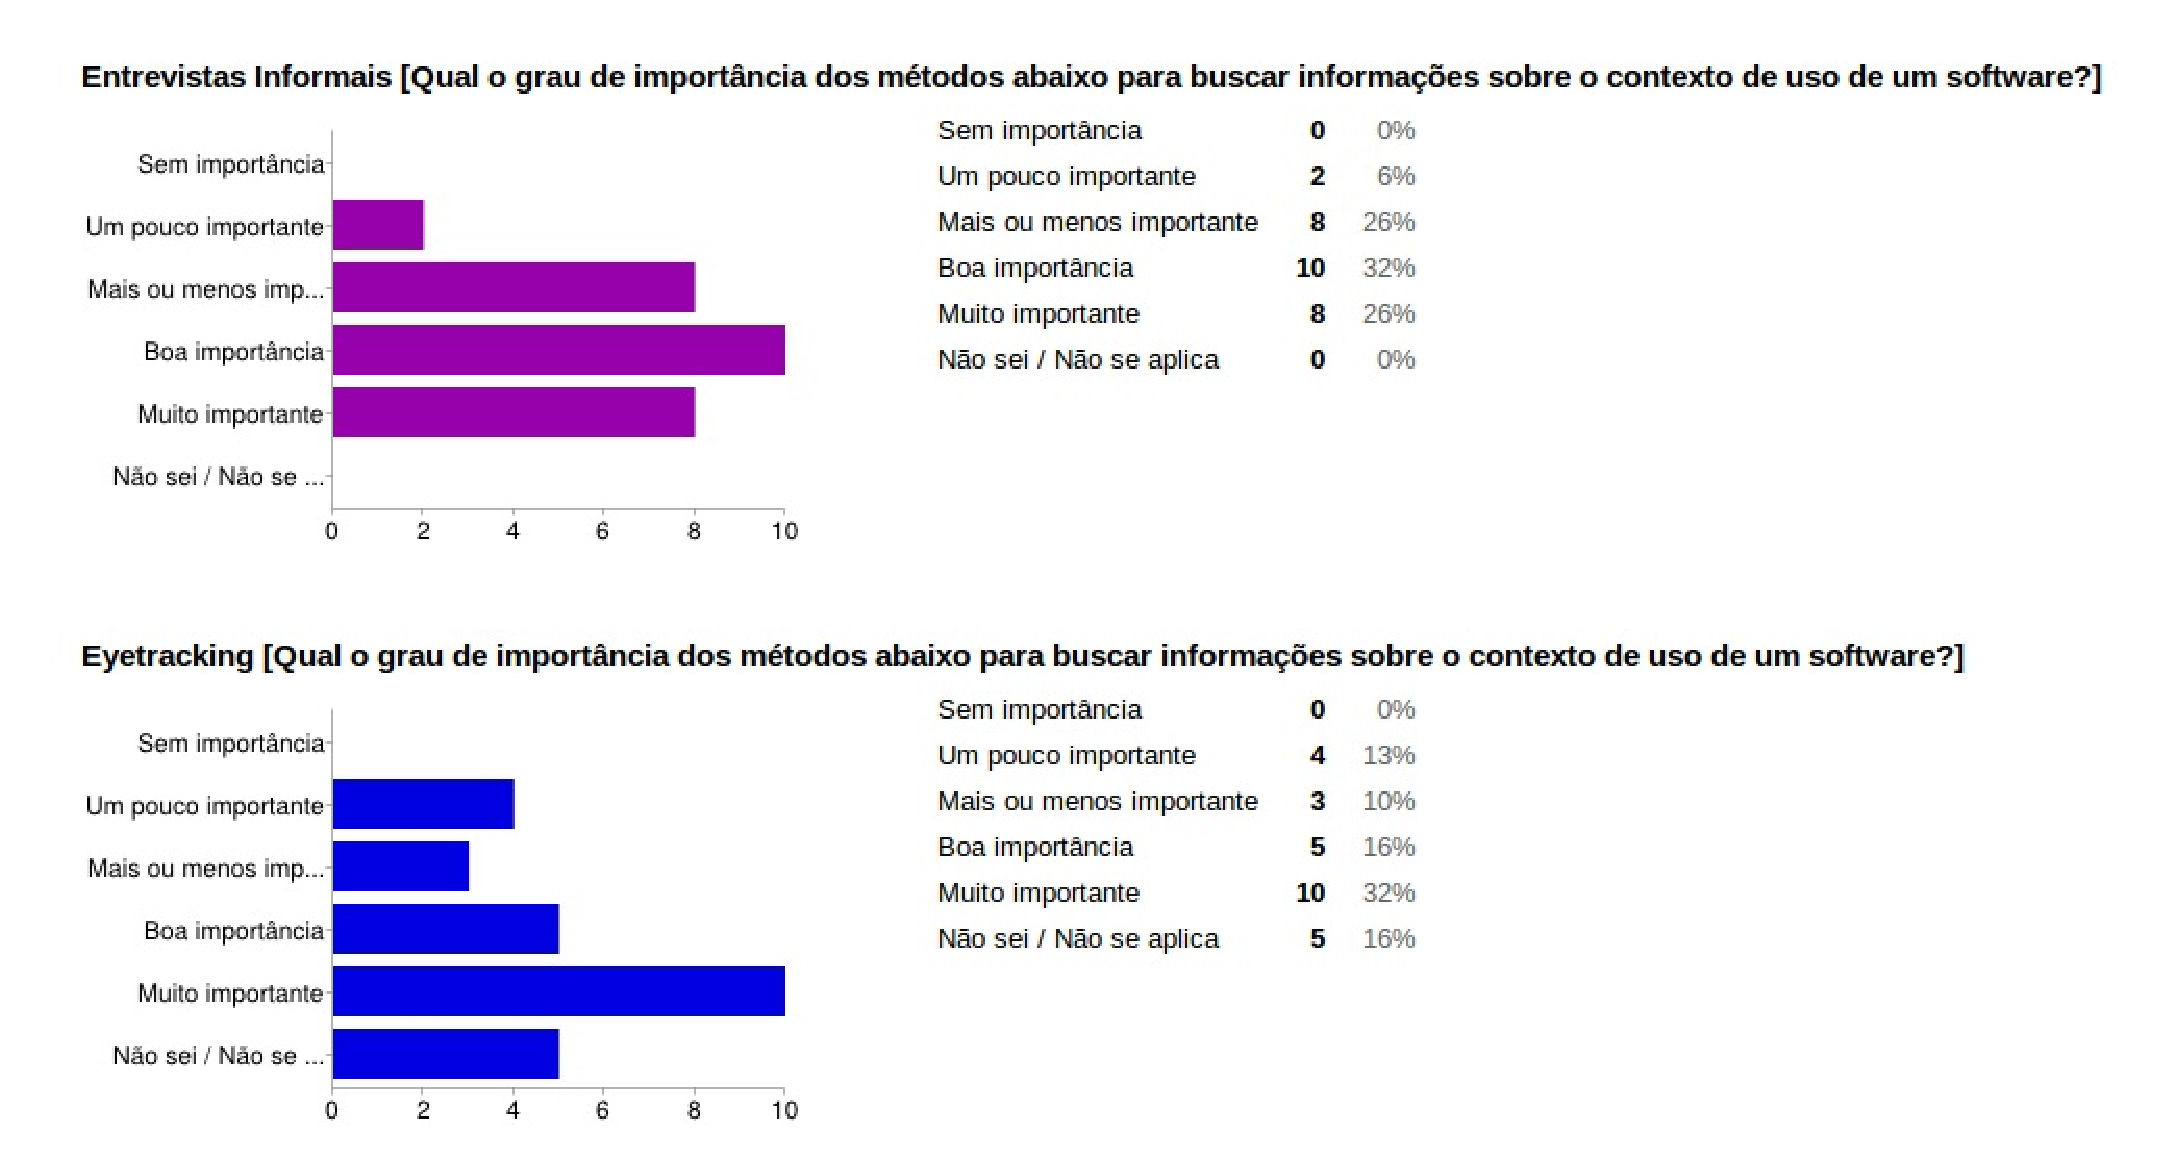
\includegraphics[keepaspectratio=true,scale=0.50]
      		{figuras/analise2.eps}
    	\label{check04}
		\caption{Técnicas de análise - Entrevistas Informais e Eytracking}
	\end{figure}

	32\% dos pesquisados informaram que a técnica de Eytracking é muito importante e 16\% não sabiam ou não aplicavam tal técnica.
		
	\begin{figure}[!h]
    	\centering
    	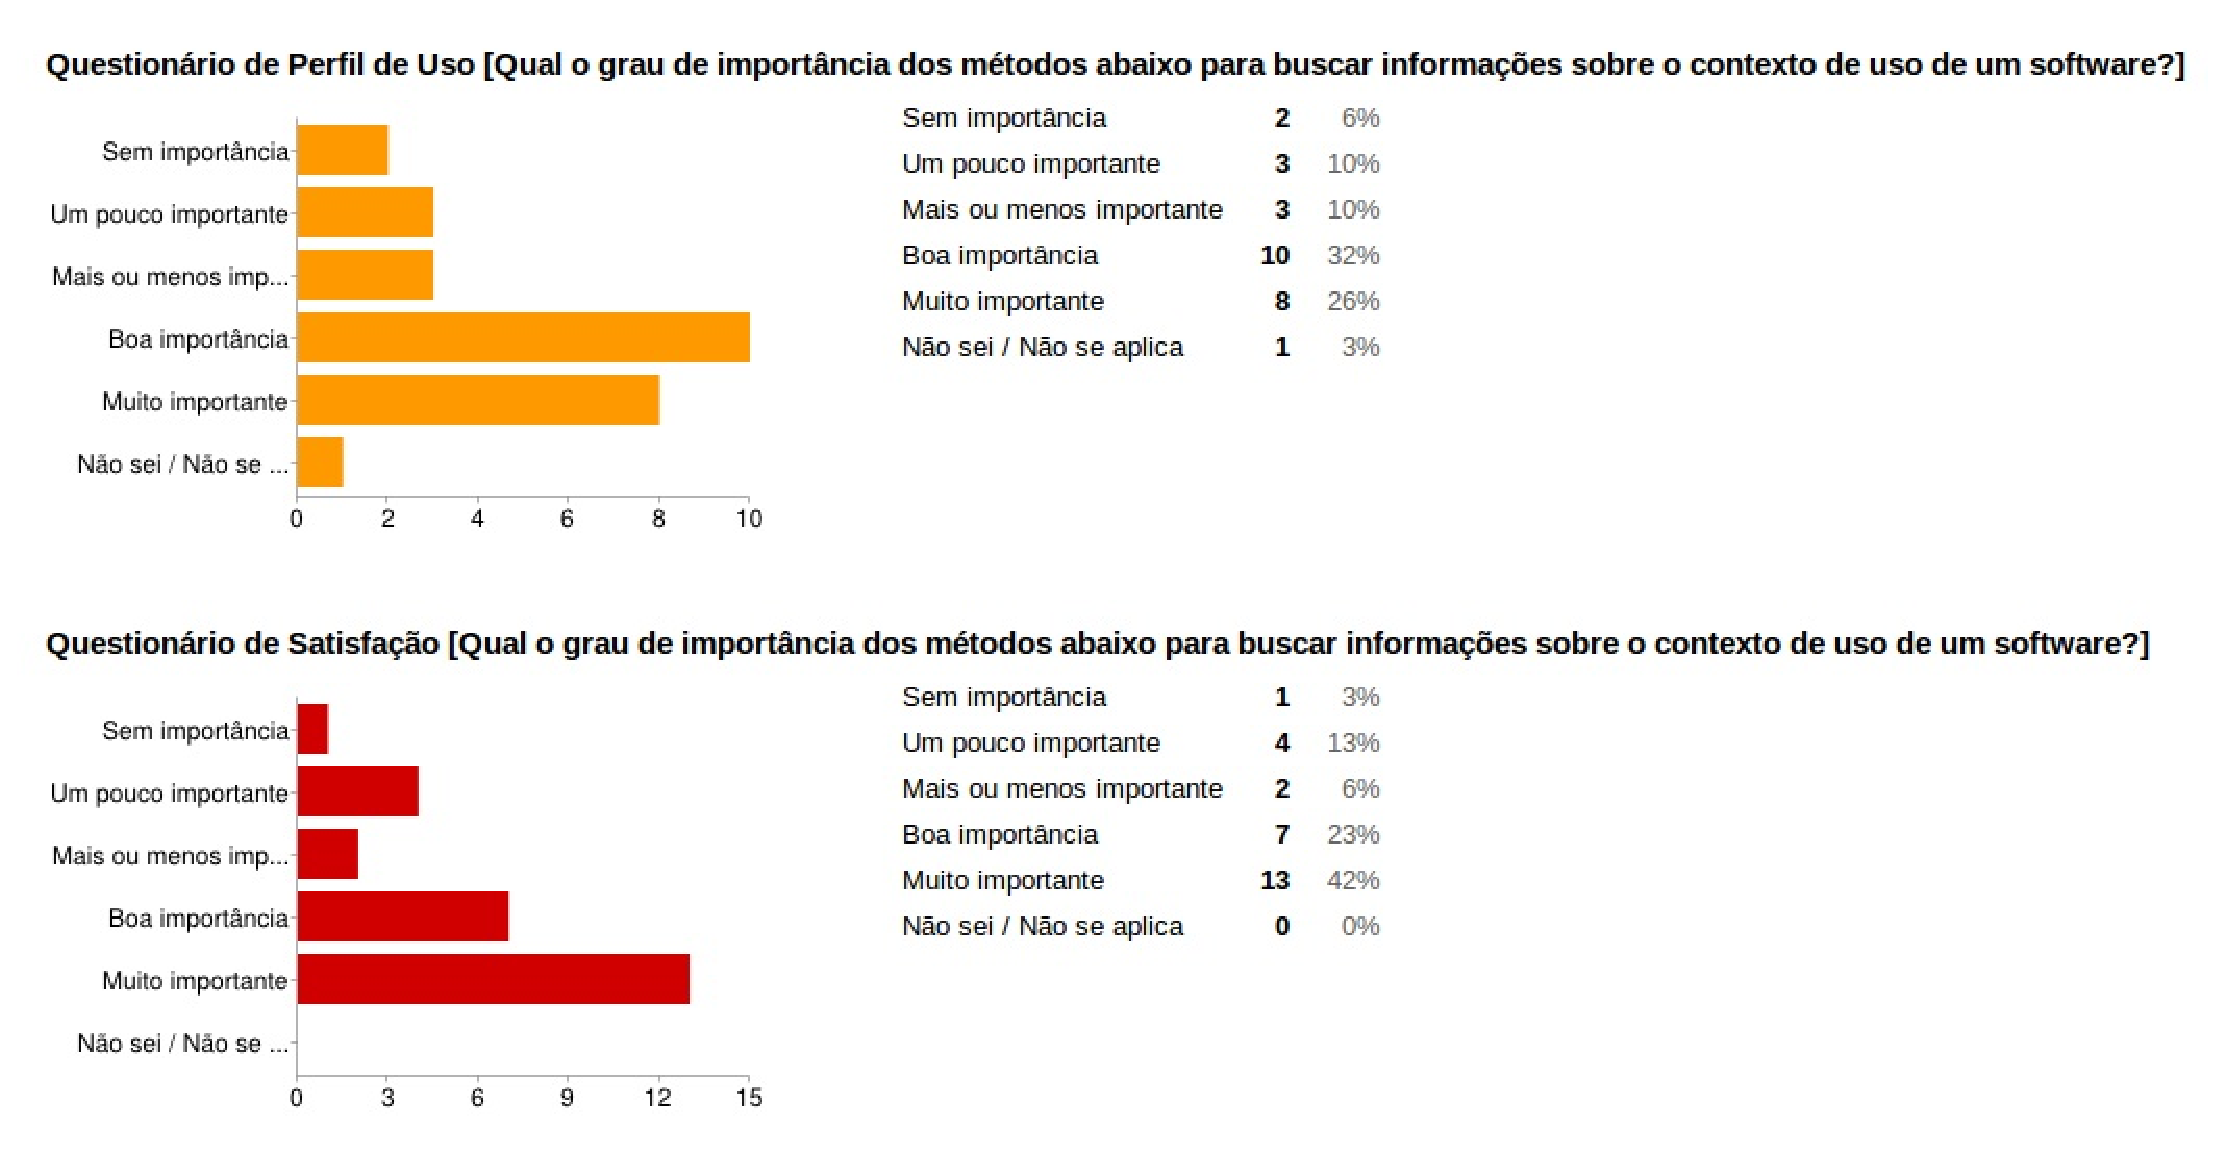
\includegraphics[keepaspectratio=true,scale=0.50]
      		{figuras/analise3.eps}
    	\label{check04}
		\caption{Técnicas de análise 'Questionários de perfil de uso e de satisfação}
	\end{figure}
	
	Os questionários de perfil de uso obtiveram boa importância, 32\%, mas alguns pesquisados, 6\% informaram que não são muito importante para realização de análises no contexto que estão inseridos.
	
	\begin{figure}[!h]
    	\centering
    	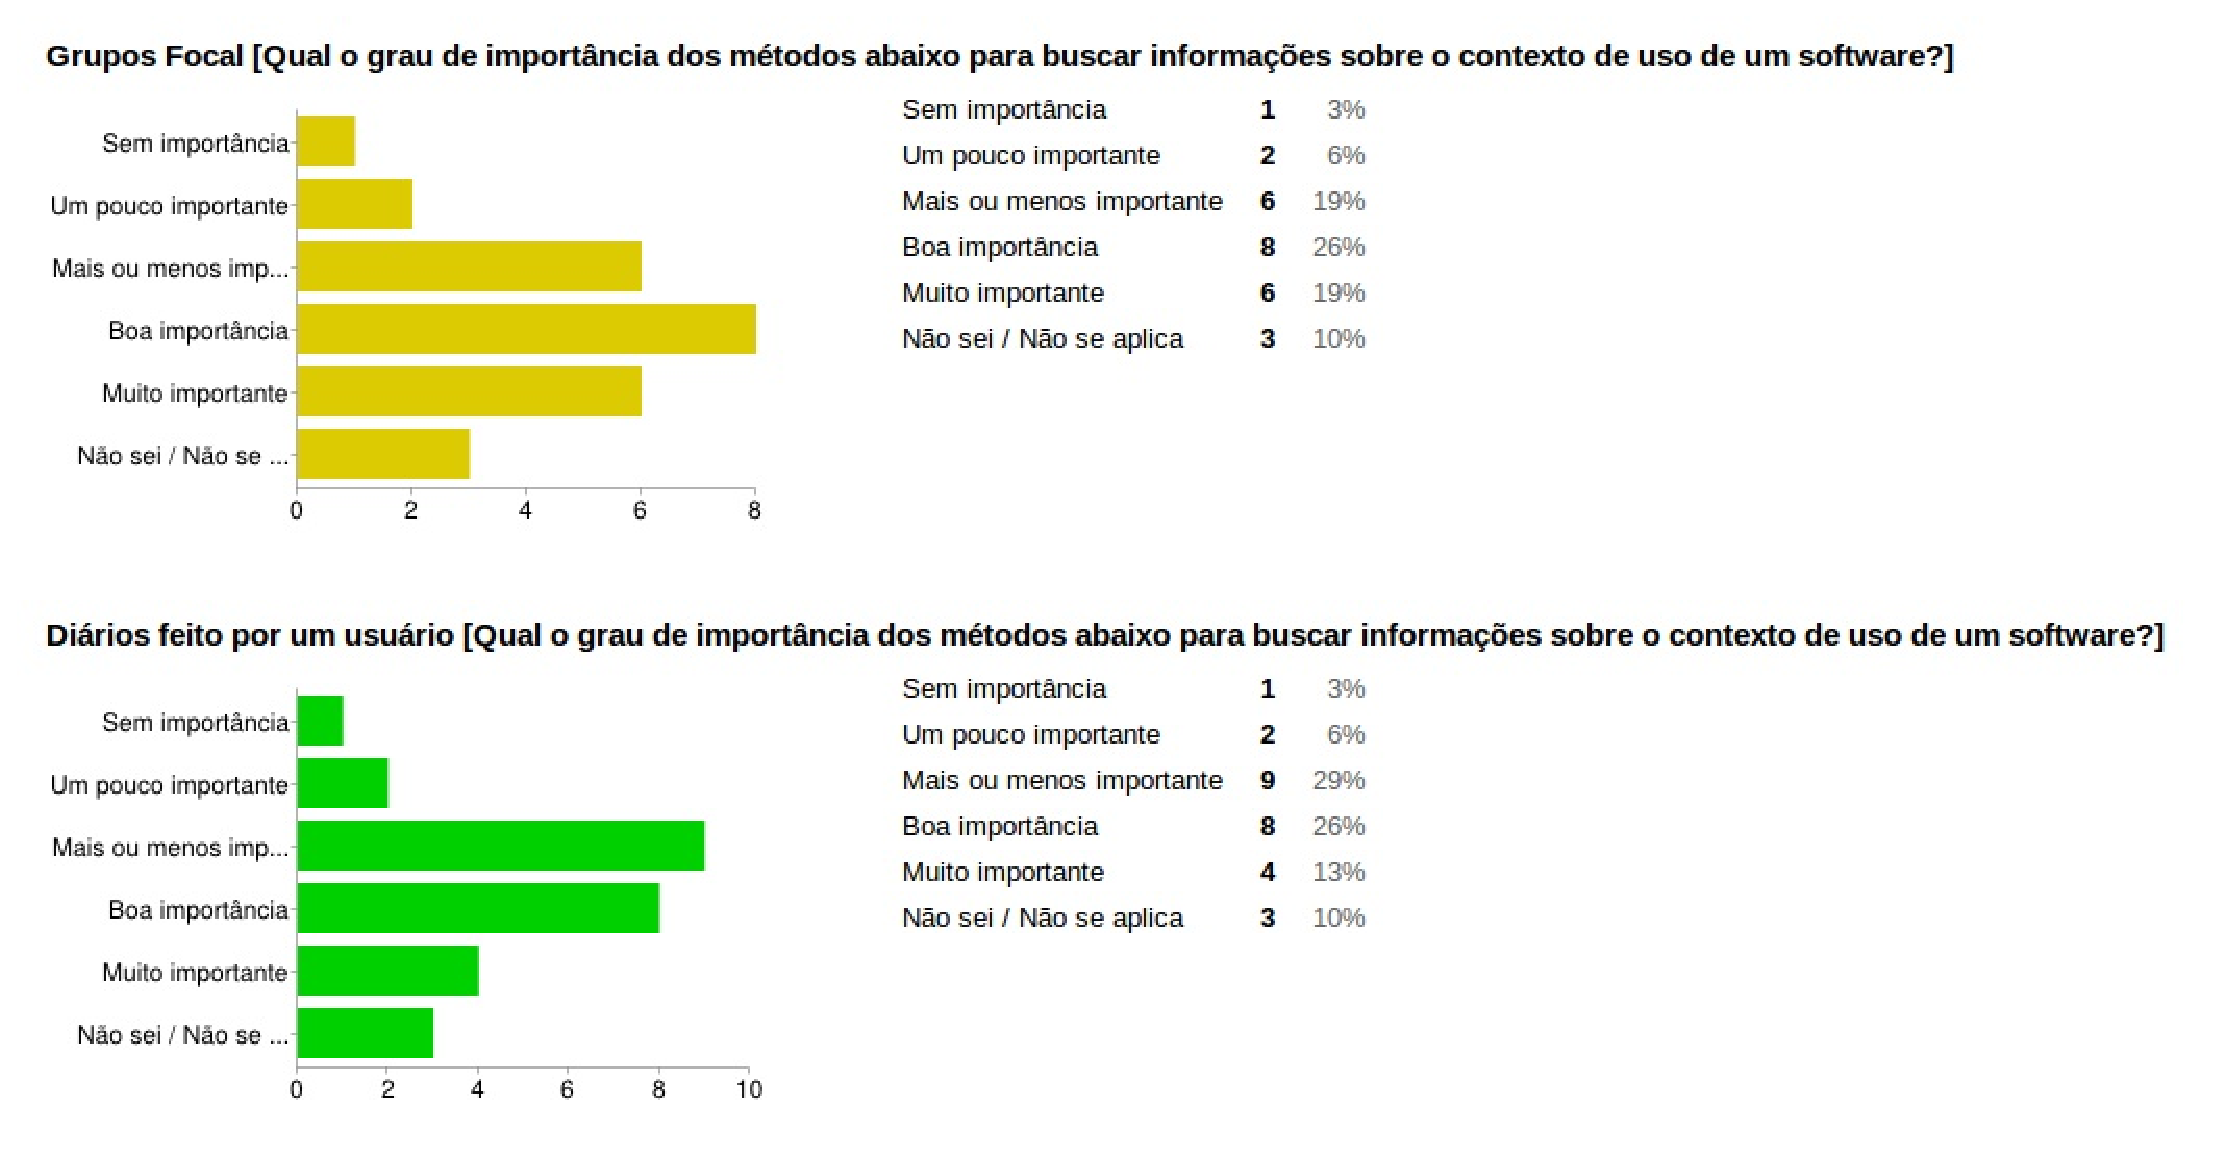
\includegraphics[keepaspectratio=true,scale=0.50]
      		{figuras/analise4.eps}
    	\label{check04}
		\caption{Técnicas de análise - Grupo Focal e Diários}
	\end{figure}
	
	
	\begin{figure}[!h]
    	\centering
    	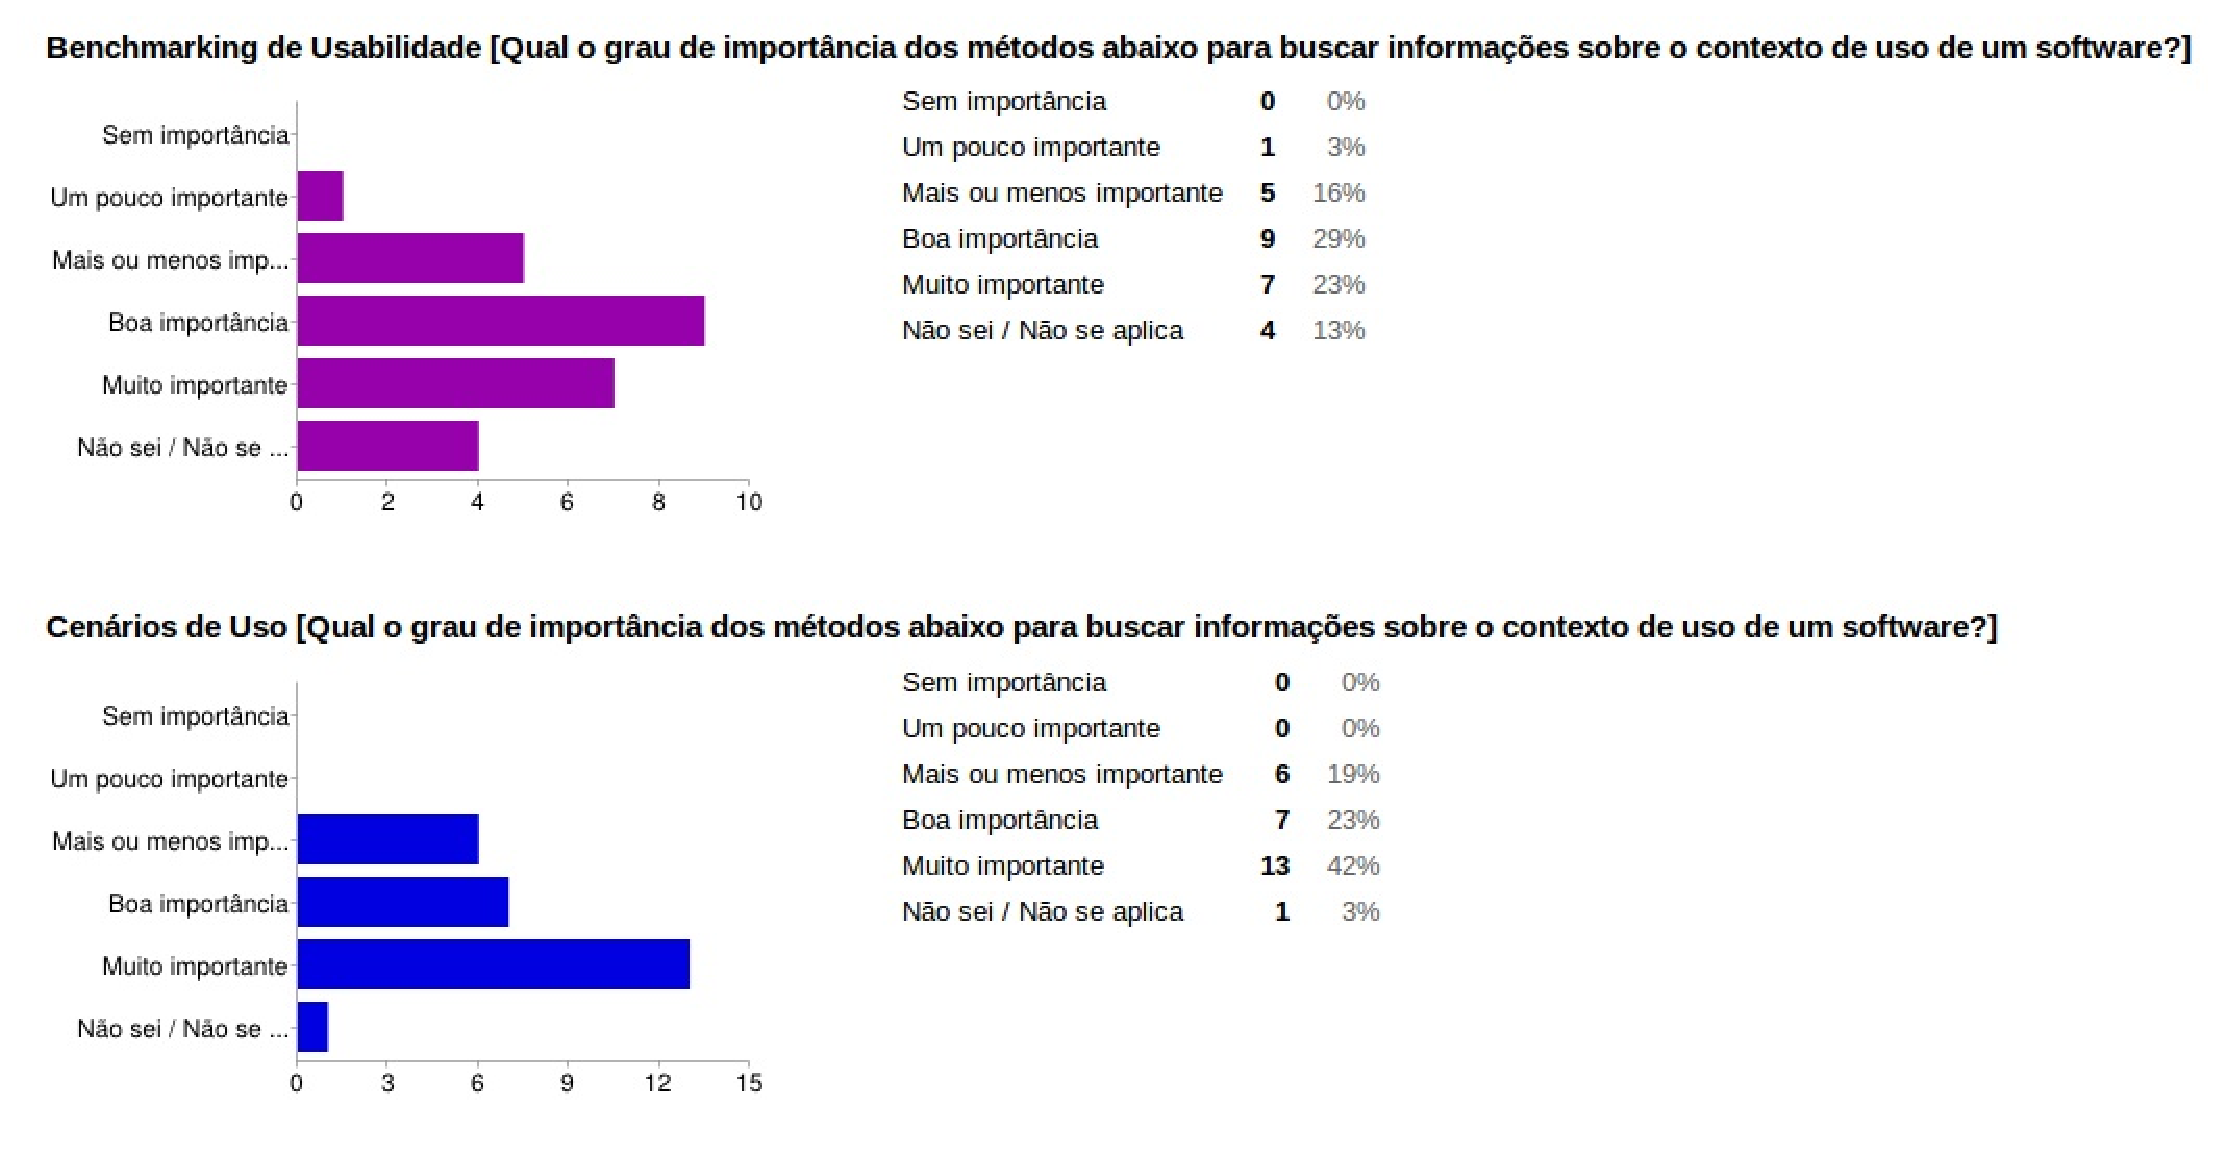
\includegraphics[keepaspectratio=true,scale=0.50]
      		{figuras/analise5.eps}
    	\label{check04}
		\caption{Técnicas de análise - Benchmarking e Cenários de uso}
	\end{figure}
		
	\begin{figure}[!h]
    	\centering
    	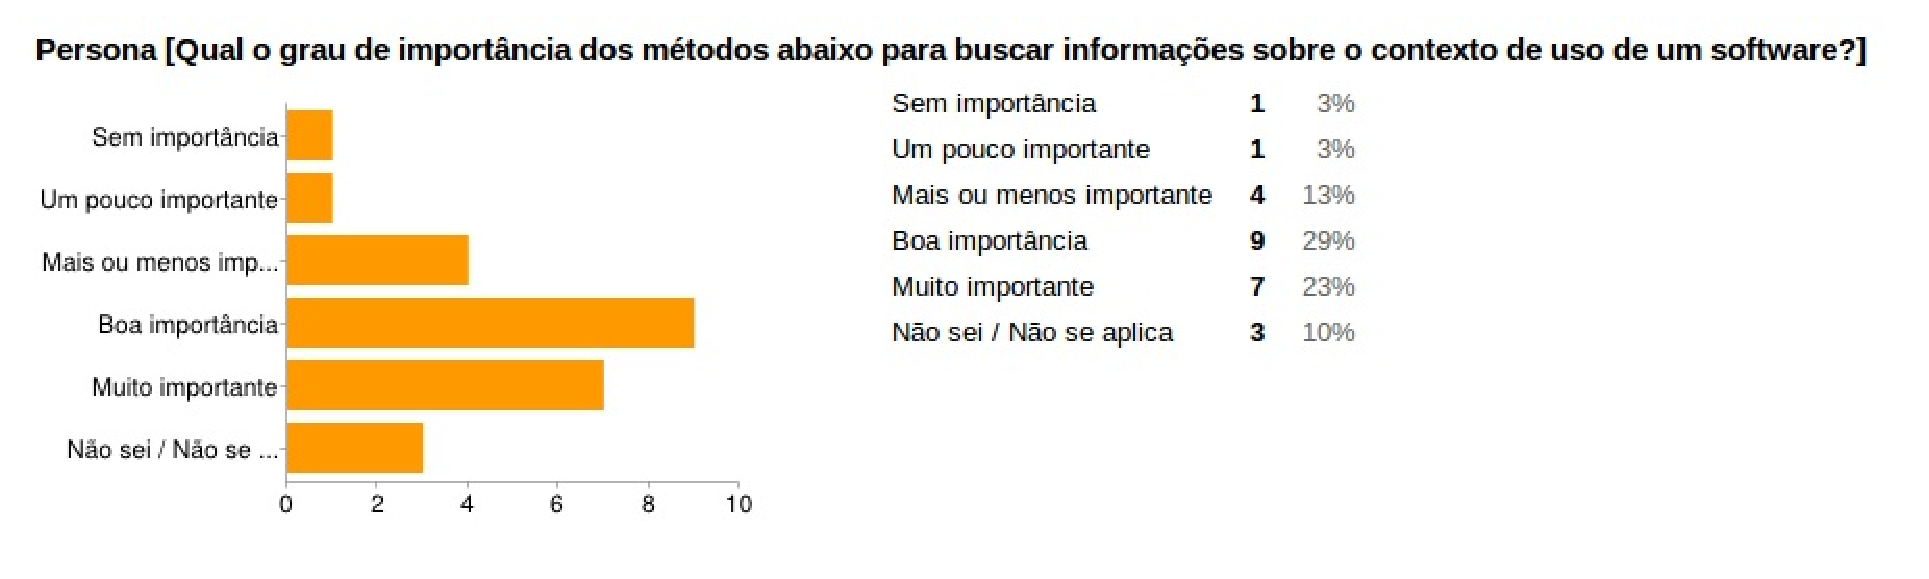
\includegraphics[keepaspectratio=true,scale=0.55]
      		{figuras/analise6.eps}
    	\label{check04}
		\caption{Técnicas de análise - Persona}
	\end{figure}

\newpage

	Os resultados abaixo são referentes as técnicas de avaliação da usabilidade.	
	
	\begin{figure}[!h]
    	\centering
    	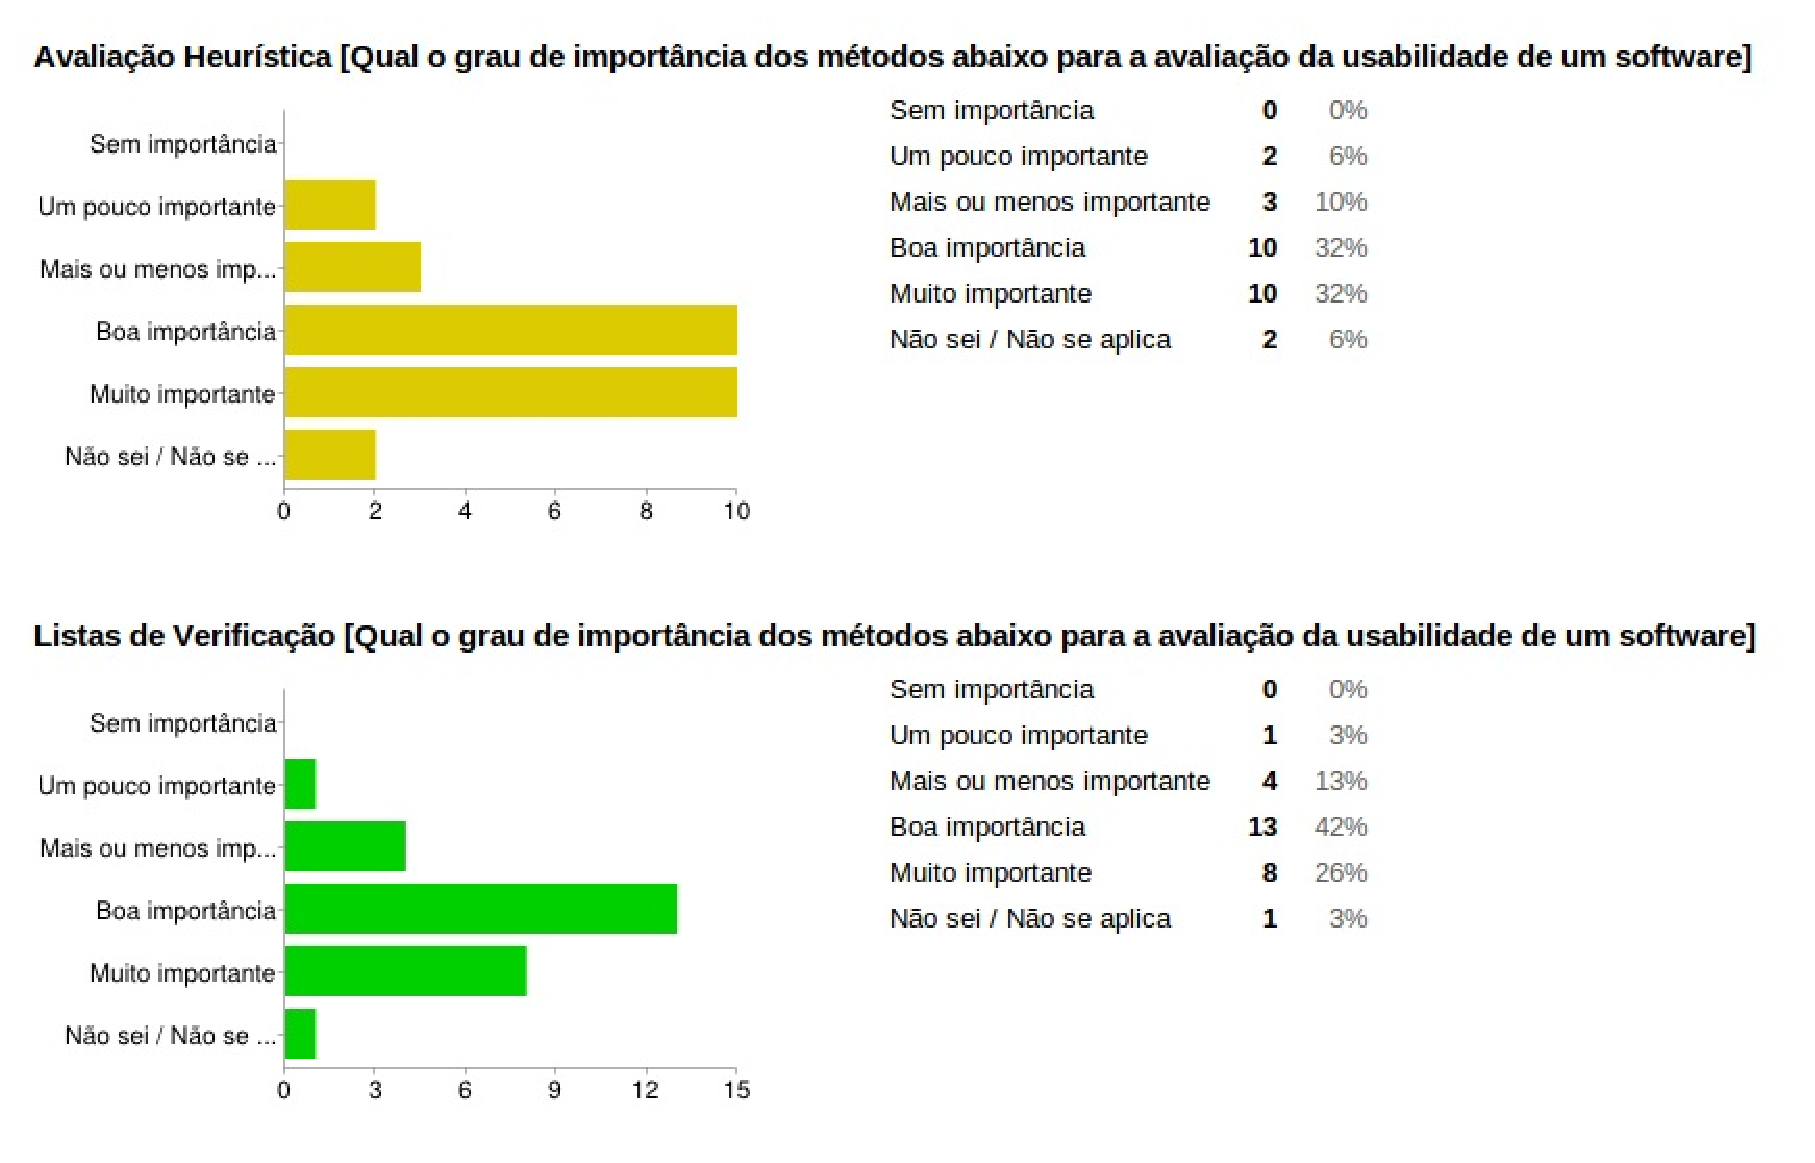
\includegraphics[keepaspectratio=true,scale=0.55]
      		{figuras/avalia1.eps}
    	\label{check04}
		\caption{Técnicas de avaliacao - Heurísticas e Listas de Verificação}
	\end{figure}
		
		Mais de 60\% informaram que as avaliações feitas por heurísticas e listas de verificação são de boa ou muita importância.
	
	\begin{figure}[!h]
    	\centering
    	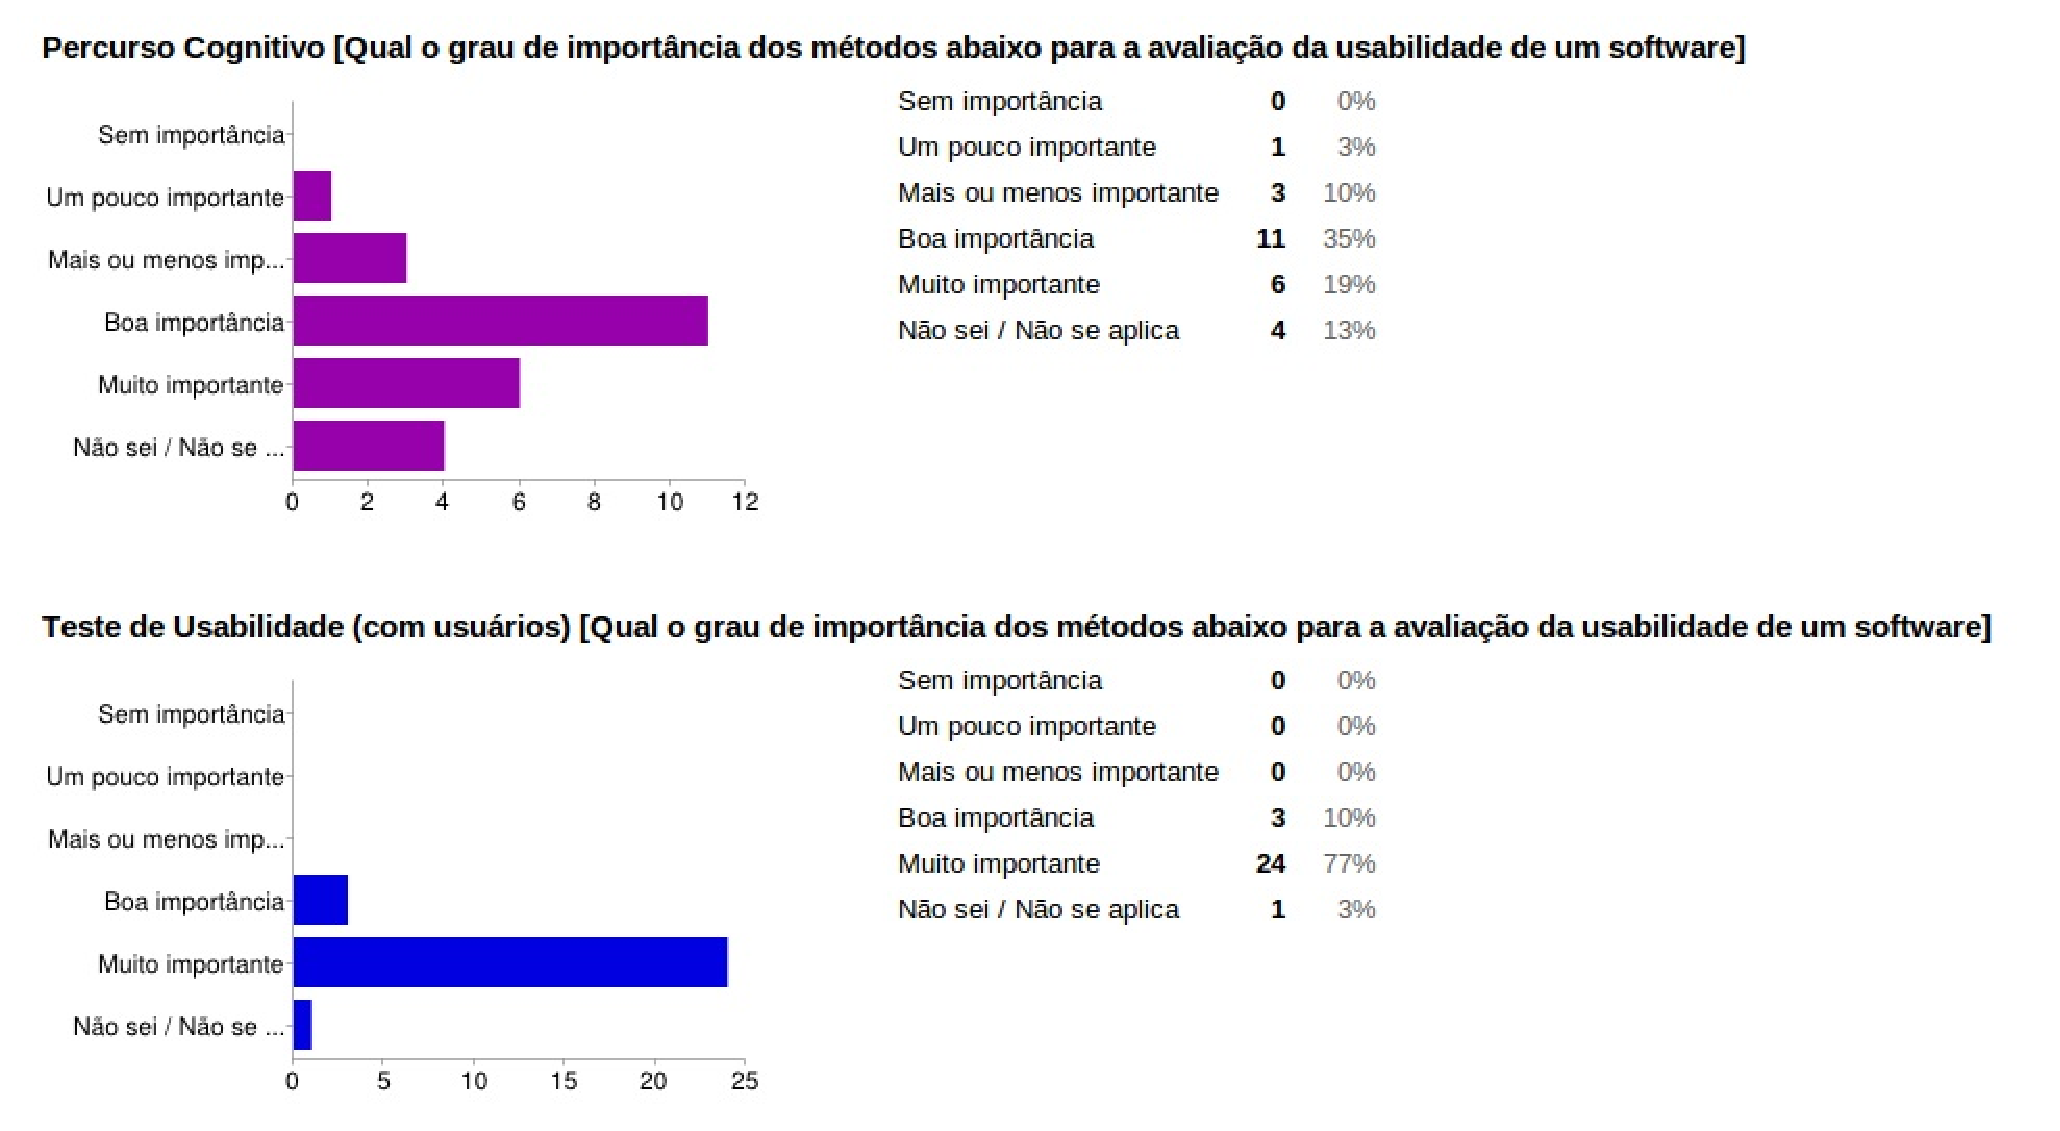
\includegraphics[keepaspectratio=true,scale=0.55]
      		{figuras/avalia2.eps}
    	\label{check04}
		\caption{Técnicas de avaliação - Percursos Cognitivos e Testes de Usabilidade}
	\end{figure}

		Os Testes de Usabilidade foram o que mais apresentaram importância para os pesquisados, sendo 77\% muito importante e 10\% boa importância.	